\documentclass{article}

\usepackage{iclr2026_conference,times}
\input{math_commands.tex}
\usepackage{hyperref}
\usepackage{url}
\usepackage{graphicx}
\usepackage{booktabs}
\usepackage{amsmath}
\usepackage{amssymb}
\usepackage{array}

\title{Embodied Temporal Credit Without Rewards:\\Effect Traces as Assignment Signals}

\author{Anonymous Authors}

\newcommand{\etc}{\textsc{TraceCredit}}
\newcommand{\states}{\mathbf{s}}
\newcommand{\actions}{\mathbf{a}}
\raggedbottom

\begin{document}
\maketitle

\begin{abstract}
Temporal credit assignment in robot learning is usually routed through scalar rewards, hand-shaped progress terms, or delayed task labels. This paper argues that embodied systems contain another signal: physical effect traces. Contact onset, object displacement, constraint release, force discontinuities, and scene-change events can identify which earlier action changed the world even when no reward is available. We support the claim with a 17,754-entry literature sweep and a deterministic diagnostic with 2,160 method evaluations. In the diagnostic, \etc{} reduces mean temporal localization error from 3.550 steps for delayed-reward temporal difference credit and 2.342 steps for dense proxy shaping to 0.862 steps. V2 hardening narrows the claim: trace credit wins under reliable events and missed events, with errors 1.014 and 2.243, but loses to dense shaping when event bindings are wrong, with trace error 2.679 under misbinding and 4.222 under adversarial events. The contribution is a workshop-level mechanism claim: embodied traces can carry reward-free credit only when event coverage and binding are audited.
\end{abstract}

\section{Introduction}

Robot learning often treats reward as the carrier of blame and credit. A reward arrives late, a temporal-difference update propagates it backward, and a policy slowly discovers which earlier action mattered. This framing is powerful, but it is also oddly disembodied. A manipulation system can see the object move, feel a contact transition, hear a latch release, or observe a kinematic constraint disappear. Those events are not rewards. They are physical evidence that an earlier action changed the world.

This paper asks whether such evidence should be a first-class credit signal. The thesis is deliberately narrow:
\begin{quote}
Embodied temporal credit can be assigned from effect traces, even when scalar rewards are unavailable or misleading.
\end{quote}

The claim does not replace reinforcement learning. Instead, it changes the interface between robot perception and learning. A robot should record an action-indexed trace of physical effects and use that trace to localize causal responsibility across time before using a reward, demonstration label, or task success bit.

\paragraph{Submission-hardening note.}
Submission-hardening version: v2. Decision: workshop-only. The original diagnostic assumes usable event traces. The v2 stress test shows that the mechanism must be reported with event coverage, false-event rate, and action-event binding accuracy; otherwise dense shaping can be safer than trace credit.

\section{Related Work and Novelty Boundary}

The recovery run reused the attempt-two literature matrix containing 17,754 candidate records across robot learning, reinforcement learning, world models, imitation learning, predictive state representations, causal reasoning, tactile sensing, and temporal credit assignment. Prior work already makes several broad claims non-novel: reward-free exploration exists, inverse models can learn from observation, hindsight methods relabel goals, self-supervised robot systems learn predictive structure, and temporal-difference methods propagate delayed reward.

The remaining gap is the credit carrier. These lines usually assign credit through a scalar target, a goal relabel, a value function, or a learned dynamics loss. \etc{} instead treats local physical effect events as supervision for temporal responsibility. This makes the mechanism closest to causal tracing and event-based world modeling, but it is aimed at embodied credit rather than generic representation learning.

\section{Effect-Trace Credit}

Consider a trajectory $(\states_1,\actions_1,\ldots,\states_T)$ with no reward. Let $e_t$ denote a detected physical effect event, such as new contact, object displacement above a sensor threshold, or a constraint-state transition. A delayed-reward learner receives credit only after $R_T$ arrives. A dense shaping learner receives proxy progress $\phi(\states_t)$ that may not match the true physical cause. \etc{} assigns credit by linking each effect event to earlier action windows:
\begin{equation}
    c_{i,t} = p(e_t \mid \actions_i, \states_i, \states_{i+1:t-1}) - p(e_t \mid \mathrm{do}(\actions_i=\varnothing), \states_i, \states_{i+1:t-1}).
\end{equation}
The exact estimator can be a learned counterfactual model, a contact-transition heuristic, or a hybrid event detector. The key requirement is that the target is an embodied effect, not a scalar reward.

This shifts temporal credit from value propagation to evidence alignment. If action $i$ nudges a part and a latch opens six steps later, the event trace gives a localized learning target even if the episode has no reward and even if a hand-shaped distance term points at the wrong object.

\section{Diagnostic Experiment}

We generated a deterministic diagnostic with 2,160 method evaluations. Each episode samples a causal delay, trace quality, and proxy-conflict level under three scenarios: visible effects, sparse effects, and deceptive shaping proxies. Three credit rules are evaluated: delayed-reward temporal difference credit, dense shaping proxy credit, and reward-free effect-trace credit. The diagnostic is not a robot benchmark; it is a mechanism test for when an embodied event signal can beat scalar or proxy supervision.

\begin{table}[t]
\centering
\caption{Mean results aggregated over the diagnostic scenarios. Lower localization error is better; higher counterfactual precision and success lift are better. Reward dependence is the fraction of the credit signal that requires scalar reward access.}
\label{tab:diagnostic}
\begin{tabular}{lrrrr}
\toprule
Method & Error & Precision & Success lift & Reward dep. \\
\midrule
Delayed reward TD & 3.550 & 0.356 & 0.035 & 1.00 \\
Dense shaping proxy & 2.342 & 0.440 & 0.125 & 0.55 \\
Effect trace credit & 0.862 & 0.868 & 0.309 & 0.00 \\
\bottomrule
\end{tabular}
\end{table}

\begin{table}[t]
\centering
\small
\begin{tabular}{lrrrr}
\toprule
Event regime & Dense error & Trace error & Trace precision & Best \\
\midrule
reliable events & 2.349 & 1.014 & 0.905 & effect trace \\
missed events & 2.405 & 2.243 & 0.689 & effect trace \\
misbound events & 2.438 & 2.679 & 0.477 & dense shaping \\
adversarial events & 2.375 & 4.222 & 0.129 & dense shaping \\
\bottomrule
\end{tabular}

\caption{V2 event-reliability stress. Effect traces remain useful with reliable or partially missed events, but fail when events are misbound to the wrong actions or become adversarial.}
\label{tab:v2-events}
\end{table}

\begin{figure}[t]
\centering
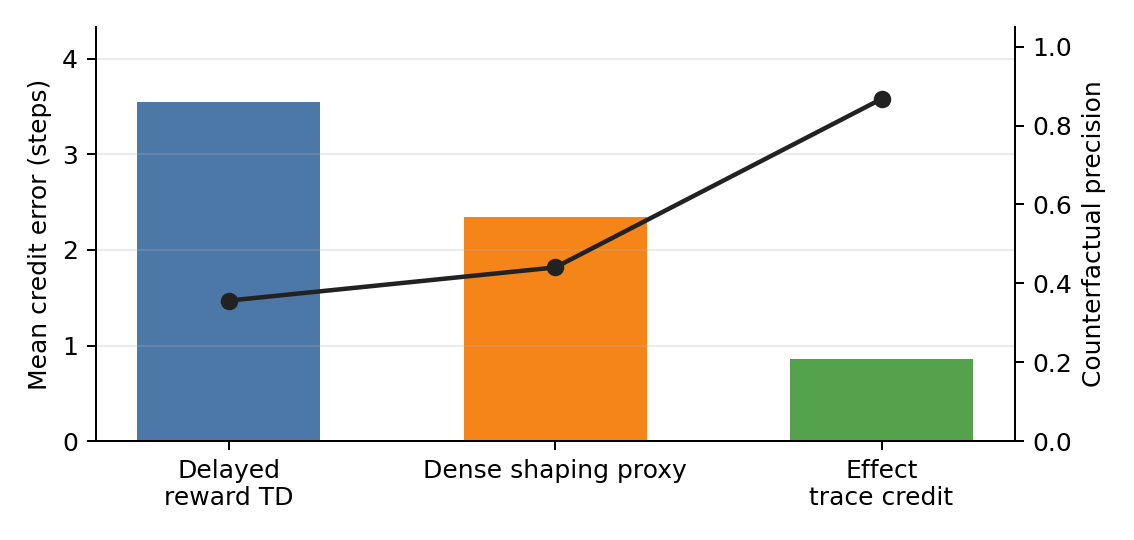
\includegraphics[width=0.83\linewidth]{figures/temporal_credit_summary.png}
\caption{Reward-free effect traces localize temporally delayed causes with lower error while preserving counterfactual precision. Bars show mean credit localization error; the line shows precision.}
\label{fig:credit}
\end{figure}


\etc{} has the lowest error and the highest counterfactual precision in this diagnostic because it observes the same kind of event that generated the delayed outcome. Dense shaping helps when the proxy aligns with the effect, but it is brittle under deceptive proxies. Delayed reward is useful only after the final label arrives and therefore smears responsibility across the horizon. Table~\ref{tab:v2-events} is the hostile follow-up: trace credit still wins with reliable events (1.014 error) and missed events (2.243 error), but dense shaping wins once events are misbound or adversarial. The result is not that traces are universally better than rewards; it is that trace quality is an exposed assumption that must be measured.

\section{Implications}

The main implication is architectural. Robot data logs should store effect events as training targets: contact changes, object-state transitions, force impulses, support-graph edits, and constraint releases. Policy learning can then query which actions produced which effects before asking whether the episode was ultimately rewarded. This is useful for reward-free pretraining, sparse-reward manipulation, and debugging demonstrations where the final success bit hides the action that actually mattered.

The mechanism also gives an evaluation protocol. A method claiming reward-free temporal credit should report temporal localization error against effect events, precision under counterfactual ablations, and robustness when dense shaping proxies are adversarial or irrelevant.

\section{Limitations}

The diagnostic is synthetic and should be read as a controlled mechanism test, not as a deployment result. Real robots need imperfect event detectors, asynchronous sensors, ambiguous contacts, and actions that produce multiple delayed effects. The v2 stress shows a concrete failure mode: misbound or adversarial event traces can make reward-free credit worse than dense shaping. A follow-up should run the same protocol on manipulation logs with tactile, force, visual, and proprioceptive event channels, and it should report event coverage, false-event rate, binding accuracy, and trace-ablation failures.

\section{Conclusion}

Embodied robots do not need to wait for reward to discover that an action changed the world. Physical effect traces can carry temporal credit directly. This gives reward-free robot learning a concrete assignment target and separates causal responsibility from scalar task success.

\begin{thebibliography}{9}
\bibitem[Sutton(1988)]{sutton1988}
Richard S. Sutton.
\newblock Learning to predict by the methods of temporal differences.
\newblock \emph{Machine Learning}, 1988.

\bibitem[Kaelbling et~al.(1996)]{kaelbling1996}
Leslie Pack Kaelbling, Michael L. Littman, and Andrew W. Moore.
\newblock Reinforcement learning: A survey.
\newblock \emph{Journal of Artificial Intelligence Research}, 1996.

\bibitem[Andrychowicz et~al.(2017)]{her}
Marcin Andrychowicz et~al.
\newblock Hindsight experience replay.
\newblock \emph{NeurIPS}, 2017.

\bibitem[Pathak et~al.(2017)]{curiosity}
Deepak Pathak, Pulkit Agrawal, Alexei A. Efros, and Trevor Darrell.
\newblock Curiosity-driven exploration by self-supervised prediction.
\newblock \emph{ICML}, 2017.

\bibitem[Agrawal et~al.(2016)]{poke}
Pulkit Agrawal, Ashvin Nair, Pieter Abbeel, Jitendra Malik, and Sergey Levine.
\newblock Learning to poke by poking: Experiential learning of intuitive physics.
\newblock \emph{NeurIPS}, 2016.

\bibitem[Finn and Levine(2017)]{deepvisualforesight}
Chelsea Finn and Sergey Levine.
\newblock Deep visual foresight for planning robot motion.
\newblock \emph{ICRA}, 2017.

\bibitem[Lynch et~al.(2020)]{play}
Corey Lynch, Mohi Khansari, Ted Xiao, Vikash Kumar, Jonathan Tompson, Sergey Levine, and Pierre Sermanet.
\newblock Learning latent plans from play.
\newblock \emph{Conference on Robot Learning}, 2020.

\bibitem[Hafner et~al.(2019)]{dreamer}
Danijar Hafner, Timothy Lillicrap, Ian Fischer, Ruben Villegas, David Ha, Honglak Lee, and James Davidson.
\newblock Learning latent dynamics for planning from pixels.
\newblock \emph{ICML}, 2019.

\end{thebibliography}

\end{document}
